\subsection{Analisis Kondisi DecMed dan PGHD}

DecMed menyediakan kerangka kerja manajemen rekam medis elektronik yang terdesentralisasi
DecMed tersusun atas tiga komponen utama:
\begin{enumerate}
    \item Mekanisme kontrol akses berbasis CapBAC melalui objek metadata akses yang disimpan \textit{on-chain} pada ledger IOTA, 
    \item Mekanisme PRE melalui Proxy Layer untuk mendelegasikan akses data yang terenkripsi tanpa harus memberikan \textit{private key}, serta 
    \item Penyimpanan \textit{hybrid} IOTA-IPFS yang memisahkan metadata akses dari \textit{payload} data klinis. 
\end{enumerate}
Kombinasi ketiga komponen tersebut memungkinkan siklus hidup RME dari pendaftaran akun pasien, pemberian akses, pembacaan, hingga penambahan entri rekam medis oleh tenaga kesehatan.

Saat ini seluruh jalur penambahan data pada DecMed berasal dari sisi tenaga kesehatan melalui kunjungan klinis di fasilitas pelayanan kesehatan (fasyankes), sementara pasien hanya bertindak sebagai pemilik data yang dapat memberi atau mencabut izin akses, bukan sebagai produsen data yang dapat mendorong informasi kesehatan ke dalam sistem secara mandiri \parencite{Purnama_2026}. 
DecMed saat ini tidak memiliki mekanisme apa pun untuk menanggulangi data yang secara aktif dapat dihasilkan pasien sendiri, seperti detak jantung, tekanan darah, atau pola aktivitas harian yang terekam oleh perangkat pasien. Akibatnya, tenaga kesehatan kehilangan gambaran kondisi pasien yang lebih lengkap pada saat melakukan evaluasi klinis, khususnya untuk kondisi yang memerlukan pemantauan berkelanjutan.
Akibatnya, rekam medis yang tersimpan di dalam ekosistem DecMed hanya mencerminkan kondisi klinis pada saat kunjungan berlangsung, dan tidak mencakup data kondisi pasien yang terjadi di antara kunjungan tersebut.
Alur sistem DecMed saat ini dapat dilihat pada Gambar~\ref{fig:decmed-original-flow}.

\begin{figure}[htbp]
    \centering
	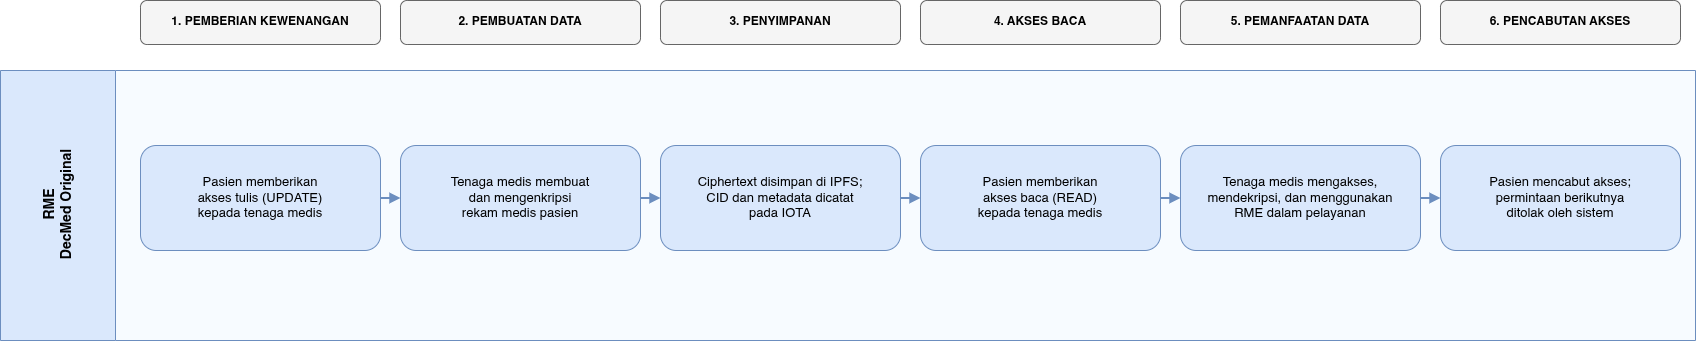
\includegraphics[width=\textwidth]{resources/chapter-3/flow-decmed.png}
	\caption{\textit{Flow} Data Rekam Medis di DecMed}\label{fig:decmed-original-flow}
\end{figure}

Kesenjangan informasi ini menjadi hambatan bagi tenaga kesehatan dalam memperoleh gambaran kondisi pasien yang lebih lengkap pada saat melakukan evaluasi klinis misalnya untuk kondisi yang memerlukan pemantauan berkelanjutan.
PGHD mencakup aktivitas harian, gejala subjektif, dan parameter fisiologis pasien, dan ketika diintegrasikan dengan sistem rekam medis elektronik terbukti membantu mengurangi \textit{information gap} antar kunjungan, mendukung intervensi lebih dini, dan meningkatkan personalisasi rencana perawatan \parencite{Tiase2020-PGHD_EHR_Integration,Cohen_Keller_Hayes_Dorr_Ash_Sittig_2016_PGHD_Integration_EHR,Mars_Scott_2022_PGHD_Healthcare}. 
Dengan menelusuri alur kerja DecMed (Subbab~\ref{studi-decmed}) dan mencocokkannya dengan karakteristik PGHD (Subbab~\ref{studi-pghd}), dapat diidentifikasi beberapa kesenjangan (\textit{gap}) antara kapabilitas DecMed saat ini dan kebutuhan integrasi PGHD\@.

Pertama, dari sisi jalur pemasukan data, seluruh aliran data pada DecMed dimulai dari sisi tenaga kesehatan dan tidak menyediakan jalur bagi data yang berasal dari perangkat pasien secara mandiri. 
Saat ini belum ada komponen yang memungkinkan aplikasi klien pasien di perangkat untuk mengumpulkan data dan mengirimkannya sebagai entri ke dalam ekosistem DecMed. 
Diperlukan suatu mekanisme untuk mengumpulkan data yang berasal dari sumber data mana saja, proses pengolahan dan pengiriman data, juga pengaksesan data PGHD \parencite{Zeng2022-Standardized-PGD}.
Hal ini menyebabkan munculnya \textbf{Gap 1}: \emph{tidak adanya jalur pemasukan PGHD dari sisi pasien, seluruh entri data pada DecMed saat ini hanya berasal dari tenaga kesehatan melalui kunjungan klinis}
% This viewpoint paper formulates the integration of PGD into clinical systems and workflow as a PGD integration pipeline and reviews the functional components of such a pipeline. A PGD integration pipeline includes PGD acquisition, aggregation, and consumption (Zeng Standardized)

Kedua, arsitektur DecMed belum mengimplementasikan mekanisme \textit{offline-first} pada klien pasien untuk menangani kasus perangkat pasien yang tidak dapat terhubung dengan sistem DecMed saat tidak ada internet. 
Dalam skenario pemantauan data rekam medis di luar fasyankes, konektivitas yang tidak stabil dapat menyebabkan PGHD yang dikumpulkan saat luring tidak pernah terkirim ke sistem \parencite{Khatiwada_Yang_Lin_Blobel_2024_PGHD_Understanding}.
Kondisi ini membentuk \textbf{Gap 2}: \emph{tidak adanya mekanisme \textit{offline-first} di sisi klien pasien agar PGHD yang dikumpulkan saat perangkat luring berisiko tidak pernah terkirim ke sistem dan hilang}.

Ketiga, dari perspektif infrastruktur penyimpanan, DecMed saat ini memanfaatkan IOTA dan IPFS untuk data klinis yang diinisiasi oleh tenaga kesehatan dengan asumsi bahwa frekuensi pembuatan entri RME mengikuti frekuensi kunjungan klinis yang relatif jarang dan berukuran moderat per entri. 
PGHD, khususnya yang berasal dari sensor \textit{wearable} dan smartphone, bersifat \textit{time-series} dengan frekuensi yang dapat mencapai beberapa pembacaan per detik dan menghasilkan volume data besar dalam periode waktu pendek. 
Mengirimkan setiap pembacaan sensor secara langsung sebagai transaksi terpisah ke IOTA Rebased tidak efisien mengingat adanya biaya \textit{gas fee} per transaksi dan batasan \textit{throughput} jaringan \parencite{FromTangleToRebased_2025}. 
Saat ini, DecMed belum memiliki mekanisme \textit{batching} yang dirancang untuk menangani volume data \textit{time-series} tinggi seperti PGHD, sehingga terbentuk \textbf{Gap 3}: \emph{tidak adanya strategi pengelolaan volume data \textit{time-series} PGHD}.

Kemudian dari segi kepercayaan dan asal-usul data, seluruh data klinis yang tersimpan di DecMed saat ini berasal dari tenaga kesehatan yang terverifikasi dan dicatat dalam konteks pelayanan klinis, sehingga memiliki tingkat kepercayaan tinggi secara medis. 
PGHD sebaliknya dihasilkan secara mandiri oleh pasien di luar pengawasan langsung penyedia layanan kesehatan, sehingga tidak secara otomatis memiliki tingkat kepercayaan yang setara dengan data klinis \parencite{Khatiwada_Yang_Lin_Blobel_2024_PGHD_Understanding}.
Meskipun demikian, PGHD tetap memiliki nilai klinis sebagai data pendukung yang melengkapi rekam medis berbasis kunjungan, selama keaslian dan keutuhan datanya dapat diverifikasi oleh tenaga kesehatan \parencite{ahima_fountain_2014_using_pghd_provenance}.
Kebutuhan akan pencatatan asal-usul, riwayat pemrosesan, dan rantai kepemilikan data sejak pertama kali dikumpulkan menjadi hal yang penting bagi PGHD\@ \parencite{Ahmed_2023_Data_Provenance}. 
Tanpa \textit{provenance} yang terdokumentasi dengan baik, tenaga kesehatan tidak dapat memverifikasi apakah suatu data PGHD benar-benar berasal dari pasien yang bersangkutan, kapan diukur, menggunakan perangkat apa, dan apakah telah mengalami transformasi selama pengiriman.
Kondisi ini membentuk \textbf{Gap 4}: \emph{tidak adanya \textit{data provenance} untuk menjamin keandalan data yang berasal dari pasien}.

Selain kesenjangan di atas yang telah diidentifikasi, integrasi PGHD juga membutuhkan adanya mekanisme yang memastikan pasien telah memberikan persetujuan eksplisit sebelum datanya dikumpulkan dan dikirimkan ke sistem. 
Tanpa mekanisme ini, pengumpulan PGHD tidak dapat dilakukan secara etis meskipun infrastruktur teknisnya sudah tersedia \parencite{Khatiwada_Yang_Lin_Blobel_2024_PGHD_Understanding}.
Data kesehatan yang dihasilkan pasien bersifat sensitif dan memerlukan perlindungan agar data hanya dapat diakses pihak berwenang, integritas data agar data tidak mengalami modifikasi tidak sah selama transmisi maupun penyimpanan, dan ketersediaan (sistem tetap dapat melayani permintaan sah meskipun terdapat lonjakan data \textit{time-series} bervolume tinggi) \parencite{Khatiwada_Yang_Lin_Blobel_2024_PGHD_Understanding}.
DecMed telah memiliki infrastruktur identitas kriptografis, akses kontrol, autentikasi, penyimpanan dan sistem terdistribusi, tetapi belum ada modul yang memanfaatkan komponen tersebut untuk menjamin kerahasiaan, integritas dan ketersediaan PGHD\@.
Hal ini memunculkan \textbf{Gap 5}: \emph{tidak adanya mekanisme penjaminan kerahasiaan, integritas dan ketersediaan untuk data PGHD pada sistem DecMed}.

\begingroup
\footnotesize
\begin{styledxltabular}{|>{\raggedright\arraybackslash}p{0.10\textwidth}|>{\raggedright\arraybackslash}X|}
    \hiderowcolors
    \caption{Rangkuman Gap Integrasi DecMed dan PGHD}\label{tab:rangkuman-gap-pghd}\\
    \hline
    \rowcolor{headerBg}
    \textbf{Kode Gap} & \textbf{Deskripsi Permasalahan} \\
    \hline
    \showrowcolors
    \endfirsthead

    \hiderowcolors
    \caption[]{Rangkuman Gap Integrasi DecMed dan PGHD (lanjutan)}\\
    \hline
    \rowcolor{headerBg}
    \textbf{Kode Gap} & \textbf{Deskripsi Permasalahan} \\
    \hline
    \showrowcolors
    \endhead

    Gap 1 & Tidak adanya jalur pemasukan PGHD dari sisi pasien, seluruh entri data pada DecMed saat ini hanya berasal dari tenaga kesehatan melalui kunjungan klinis. \\
    \hline
    Gap 2 & Tidak adanya mekanisme \textit{offline-first} di sisi klien pasien, sehingga PGHD yang dikumpulkan saat perangkat luring berisiko tidak pernah terkirim ke sistem. \\
    \hline
    Gap 3 & Tidak adanya strategi pengelolaan volume data \textit{time-series} PGHD, padahal data dari \textit{wearable} dan perangkat mobile dapat berfrekuensi tinggi dan bervolume besar. \\
    \hline
    Gap 4 & Tidak adanya mekanisme \textit{data provenance} untuk PGHD, sehingga asal-usul, waktu pengukuran, dan perangkat penghasil data tidak dapat ditelusuri dan diverifikasi. \\
    \hline
    Gap 5 & Tidak adanya mekanisme khusus untuk menjamin kerahasiaan, integritas, dan ketersediaan PGHD, meskipun infrastruktur identitas dan kontrol akses sudah tersedia di DecMed. \\
    \hline
\end{styledxltabular}
\endgroup

Kelima \textit{gap} pada Tabel~\ref{tab:rangkuman-gap-pghd} menjadi dasar perumusan kebutuhan fungsional dan non-fungsional pada Subbab berikutnya, serta menjadi acuan dalam menyusun alternatif solusi dan rancangan integrasi PGHD pada DecMed.
